%%%%%%%%%%%%%%%%%%%%%%%%%%%%%%%%%%%%%%%%%%%%%%%%%%%%%%%%%%%%%%%%%%%%%%%%%%%%%%%%
% Template for USENIX papers.
%
% History:
%
% - TEMPLATE for Usenix papers, specifically to meet requirements of
%   USENIX '05. originally a template for producing IEEE-format
%   articles using LaTeX. written by Matthew Ward, CS Department,
%   Worcester Polytechnic Institute. adapted by David Beazley for his
%   excellent SWIG paper in Proceedings, Tcl 96. turned into a
%   smartass generic template by De Clarke, with thanks to both the
%   above pioneers. Use at your own risk. Complaints to /dev/null.
%   Make it two column with no page numbering, default is 10 point.
%
% - Munged by Fred Douglis <douglis@research.att.com> 10/97 to
%   separate the .sty file from the LaTeX source template, so that
%   people can more easily include the .sty file into an existing
%   document. Also changed to more closely follow the style guidelines
%   as represented by the Word sample file.
%
% - Note that since 2010, USENIX does not require endnotes. If you
%   want foot of page notes, don't include the endnotes package in the
%   usepackage command, below.
% - This version uses the latex2e styles, not the very ancient 2.09
%   stuff.
%
% - Updated July 2018: Text block size changed from 6.5" to 7"
%
% - Updated Dec 2018 for ATC'19:
%
%   * Revised text to pass HotCRP's auto-formatting check, with
%     hotcrp.settings.submission_form.body_font_size=10pt, and
%     hotcrp.settings.submission_form.line_height=12pt
%
%   * Switched from \endnote-s to \footnote-s to match Usenix's policy.
%
%   * \section* => \begin{abstract} ... \end{abstract}
%
%   * Make template self-contained in terms of bibtex entires, to allow
%     this file to be compiled. (And changing refs style to 'plain'.)
%
%   * Make template self-contained in terms of figures, to
%     allow this file to be compiled. 
%
%   * Added packages for hyperref, embedding fonts, and improving
%     appearance.
%   
%   * Removed outdated text.
%
%%%%%%%%%%%%%%%%%%%%%%%%%%%%%%%%%%%%%%%%%%%%%%%%%%%%%%%%%%%%%%%%%%%%%%%%%%%%%%%%

\documentclass[letterpaper,twocolumn,10pt]{article}
\usepackage{usenix_2020_09}

% to be able to draw some self-contained figs
\usepackage{tikz}
\usepackage{amsmath}
%\usepackage[demo]{graphicx}
\usepackage{caption}
\usepackage{subcaption}
\PassOptionsToPackage{hyphens}{url}\usepackage{hyperref}

% inlined bib file
\usepackage{filecontents}

% add algorithm
%\usepackage{algorithm}
%\usepackage{algpseudocode}
%\usepackage[colorinlistoftodos]{todonotes}
%\usepackage{comment}
%\usepackage{gensymb}


%-------------------------------------------------------------------------------
\begin{document}
%-------------------------------------------------------------------------------

%don't want date printed
\date{}

% make title bold and 14 pt font (Latex default is non-bold, 16 pt)
\title{\Large \bf Is the Synthesized Scene in Autonomous Driving Realistic?}

%for single author (just remove % characters)
\author{
{\rm Elaine Yao}\\
University of British Columbia
% copy the following lines to add more authors
% \and
% {\rm Name}\\
%Name Institution
} % end author

\maketitle

%-------------------------------------------------------------------------------
 \begin{abstract}
%-------------------------------------------------------------------------------
\textbf{For Autonomous Vehicles(AVs), sensor perception is safety-critical. 
	Failures in object detection can cause disasters. 
	Despite various prior works on adversarial 3D physical attacks in AVs, all of them are simulating placing obstacles on the road with a synthesized scene.
	However, the rendering functions to generate the synthesized scenes may not be able to ensure the physical consistency between the obstacle and the background.
	The real-world sensor perception is much more complicated. In this project, we present the study of authenticity issues of rendering-based synthesized scenes in AV systems.
	We evaluate this by generating different synthesized scenes and testing the performance of the neural network on them.
	This allows us to quantify how realistic these scenes are and understand the impact of physical consistency in the scene on the effectiveness of generated adversarial objects.}


\textbf{We design a comprehensive test suite aiming at evaluating whether the method to integrate a 3D object in the road background is realistic or not.
	We adopt empirical approaches that address four main design challenges: 
	various impact factors, physical environment consistency, domain-specific metrics, and automated pipeline.
	We evaluate the synthesized scene with our test suite in representative open-source industry-grade AD system object detection models with real-world driving scenarios.
	We also choose a state-of-art adversarial 3D physical attack for evaluation in malicious cases.
	Our results show that most synthesized scenes are not realistic enough so the object detection fails to detect the obstacles in it.
	Such a phenomenon can reduce the effectiveness guarantee of generated 3D adversarial attacks in the physical world.}




 \end{abstract}


%-------------------------------------------------------------------------------
\section{Introduction}
%-------------------------------------------------------------------------------
% In introduction, I must be very clear about the question that I want to tackle. 
% It's not about the feasibility of the attack, but about, is the simulation for 3d physical adversarial attacks realistic enough?
% Here I can also add some anaysis in physical adversarial simulation from other papers(cite, search for citing figures from other source)

Autonomous Vehicles(AVs) can sense the surrounding environment and move safely with little human input.
They are playing an important role in future transportation. Large companies such as Google,
Uber\cite{1} are racing to develop AVs and some high level , such as level 4 self-dirving cars have already been deployed on the road. 
Level 4 is considered to be fully autonomous driving. It can handle complex urban driving situations without driver intervention. 
A fundamental part in autonomous driving system is perception.
It uses sensors\cite{17} such as cameras, LiDARs, Radars, IMU(Inertial
Measurement Unit) and GPS to know the physical environment and react accordingly. Among them, perception sensors
including cameras and LiDARs provide the obstacle and traffic sign information to AVs to avoid wrong decisions like
collision and violating traffic rules, etc. 
Failures in perception can pose a threat to the safety of self-driving. 
In 2020, a tesla car in autopilot mode collided with an overturned truck as it failed to detect it.
Therefore, multiple prior works have been studying the security of these perception sensors.

Prior work has shown that AVs are vulnerable to attacks
towards camera \cite{7, 9, 23} or LiDAR sensors \cite{4, 6, 19, 25}.
Adversaries can change the texture of 2D image \cite{23}(e.g.,
stop sign) or add well-designed adversarial patches\cite{9} to
mislead the cameras. They can also inject laser\cite{6} to spoof
the LiDAR sensors.

All of these studies, however, are limited to attacks with synthesized background, 
i.e., integrating the adversarial object with the road background through rendering functions instead of realistic simulation\cite{23, 25, msf-adv, black-lidar, 19}.
In order to simulate the scenario where a 3D vehicle is put in the road, 
these work will synthesize the attacked-influenced sensor perception, for example, the point clouds by LiDAR and images by camera with respective 3D rendering functions.
These rendering techniques provided by computer graphics can simulate the real sensor functions
 but still lack comprehensive consideration in sensing the environment due to the simplicity of its model.
By contrast, sensor perception in physical world can integrate more information such as light condition, realistic texture of adversarial objects, reasonable positions.
Although most recent works in adversarial attacks will evaluate their methods in physical world to show the effectiveness and feasibility,
they use the synthesized method to generate the malicious objects for faster speed.
The assumption that the synthesized attack-influenced background is realistic should be believed to hold in general\cite{msf-adv} and thus examining the effectiveness of this method is an urgent call.

This project presents a study on evaluation of the reality of synthesized backgrounds in AD perception systems today.
We test the above rendering-based simulation assumption by evaluating the neural network performance on these integrated sensor perception outputs used in the state-of-art adversarial attack work.
This allows us to gain a solid understanding of how much authenticity guarantee the use of synthesized background can provide as a realistic simulation way to generate effective adversarial objects.
Specifically, we consider physical 3D objects as the attack vectors for real-life feasibility and examine the performance of object detection neural network models deployed in real AV systems on the synthesized scenes.

Even though previous works have designed perception rendering functions for camera and LiDAR, we find that simply feeding them with different objects and backgrounds won't meet our requirements.
First, we need to identify the factors in the synthesized scene that might influence the detection accuracy of the neural network.
For example, the object detection model may find it difficult to detect an object which is far from away the sensor.
Also, the color of the obstacle is similar to surrounding environment so that it's hidden from the neural network.
Second, physical consistency between the obstacle and the driving background should be maximum guaranteed. 
No matter where we put the obstacle, it should stand on the road instead of floating in the air or hitting the ground.
It should also follow the shadow caused by sunlight.
Third, to quantify the authenticity of the synthesized scene, we need to come up with domain-specific metrics.
The previous works use different metrics to measure whether their adversarial obstacle achieves the goal and lack unified standard,
which makes it difficult to provide fair and reasonable metrics.
Fourth, we need to develop an automated pipeline for generating different synthesized scene, evaluating the neural network performance in the scene without attack as well as with attack.
Manually adjusting the parameters can take a long time and it's hard to do large scale analysis.

Towards this end, we design an automatic and comprehensive synthesized scene test suites, which addresses the challenges above and thus provides evaluation for the authenticity of these rendering methods.
Through preliminary experiments, we choose different driving backgrounds, 3D obstacle properties(including the color, shape and texture) and the interaction between the background and the obstacle, 
e.g., the relative position, as the impact factors and serve them as the parameters to adjust.
The attackers assumed in the previous work can just place an object on the road as simulated in the synthesized scene.
To systematically generate realistic scene, we adopt camera imaging theory to adjust the height of the object so that it's standing on the road. 
Light condition is considered to comply with the driving background. 
Also, we start with normal obstacle which can be obtained from life easily, e.g., a common chair.
Under these test settings, we address design challenge 3 by considering the correctness of bounding box of detected object, object class and its corresponding confidence score.
We extract these by parsing the output of object detection neural network. 
Also, we use these as building blocks to compute the overall scores for authenticity of the scene.
In the end, we developed automated pipelines for selecting different factors and evaluating the detection performance under benign and malicious cases.

We evaluate the scene synthesizing method in MSF-ADV\cite{msf-adv} and choose the image object detection neural network model in Autoware.AI\cite{autoware}, which is representative for current AD systems.
We also choose the attack in MSF-ADV\cite{msf-adv} to generate adversarial 3D objects which can both fool the camera and LiDAR object detection models.
We select 3 shapes of chairs from McGill 3D Shape Benchmark\cite{McGill} and evaluate each on 5 real-world driving scenarios from the KITTI dataset\cite{kitti}.
60 different scenes are synthesized and evaluated. 
Our results show that the benign obstacle in the synthesized scene fail to be detected in all the test settings.
We also find that for the attack strategy generating the adversarial object, if the benign object fails to be detected in the first place, 
it's also hard to generate effective adversarial obstacles. 
What's more, in this situation, it's hard to provide guarantee that the generated adversarial object is effective in physical world.

In summary, this work makes the following contributions:
\begin{enumerate}
	\item We study the authenticity of synthesized scenes in AD perception systems. 
	We successfully design a comprehensive test suite aiming at evaluating the whether the method to integrate an 3D object in the road background is realistic or not.
	\item We adopt empirical approaches that address four main design challenges: 
	various impact factors, physical environment consistency, domain-specific metrics and automated pipeline.
	\item We evaluate the synthesized scene with our test suite in representative open-source industry-grade AD system object detection models with real-world driving scenarios.
	We also choose state-of-art adversarial 3D physical attack for evaluation in malicious cases.
	Our results show that most synthesized scenes are not realistic enough so that the object detection fail to detect the obstacles in it.
	Such phenomenon can reduce the effectiveness guarantee of generated 3D adversarial attacks in physical world.
\end{enumerate}

While rendering the obstacle into the road background is a general way of generating adversarial 3D obstacles, 
prior works lack the realistic validation of the synthesized scene. 
In this project, we try to evaluate it by measuring the neural networks performance under different settings.
We hope that our findings can inspire more future related research to validate their rendering process in AD perception when designing the 3D adversarial obstacles.


%To defend the aforementioned attacks, researchers designed
%transformation for perceived inputs from camera\cite{13} and LiDAR\cite{22} sensors individually. Multiple Sensor Fusion(MSF)
%algorithms are also proposed to integrate inputs from cameras and LiDARs to produce correct output based on the
%unattacked sensors.
%
%However, an important and widely accepted assumption in
%MSF is there is at least one clean sensor\cite{msf-adv}.
%
%This assumption is approved to fail at specific situations
%by Cao et al. \cite{msf-adv}. They observed that different shapes of a 3D
%object can spoof both LiDARs and cameras with the change
%of point position and pixel valuesc\cite{msf-adv}. Also, the generated 3D
%objects are stealthier and more robust than previous work. As
%no safe sensor exists under this attack, the MSF algorithm doesn’t
%have reliable sensors to trust. Most recovering-based defenses only work in one kind of sensor attack and thus fail to
%have good performance under this scenario. Therefore, 
%in the experiments, the car didn’t detect the adversarial obstacles and crashed into it.
%
%We observe that defense against attacks to both cameras
%and LiDARs is urgently needed to secure AVs. Even though
%some prior works\cite{if-defense, 22, 24} have studied 3D objects adversarial defenses. They are targeting pure neural networks
%instead of a real AV system. The object detection in a real AV
%system consisting of input pre-processing(e.g., format transformation, feature generation, etc.), neural network model,
%post-processing(e.g., clustering, multiple sensor fusion, etc.).
%Also, static and general 3D objects are considered in prior
%works rather than moving and traffic-related objects. Thus,
%their methods can’t be directly applied to the attack we’re
%targeting.
%
%Our motivation comes from the previous defenses that remove perturbations from the corrupted inputs\cite{8, 14},
% or take the majority vote
%from randomly transformed image\cite{12} against2D images and 3D objects adversarial attacks. 
%The main idea behind these defenses is to do transforms on
%the perception input and remove the malicious characteristics
%generated by the attacker. 
%
%Therefore, in this work, we aim to smooth the noisy surface of obstacles with this latest 3D point cloud reconstruction network - IF-Defense\cite{if-defense}.
%IF-Defense\cite{if-defense} aims to recover the surface of 3D objects with the awareness of geometry property and uniform distribution of the points.
%However, it's only trained and tested in the dataset containing single 3D objects.
%Its performance in working in real AV perception is unknown.
%Moreover, directly applying IF-Defense\cite{if-defense} may result in unnecessary computational overhead as 
%not all the 3D perception needs recovery. 
%For example, in a wide open area, the majority of the perception is road and only a small part is the obstacles.
%
%Based on this, we further propose a lightweight segmentation algorithm, aiming to provide a rough location for the areas to be recovered.
%The intuition for this algorithm is, we observe that due to laser imaging in the LiDAR system, a blank shadow is formed after the obstacle.
%Usually, the number of points in the obstacle area is much larger than that in road areas.
%And the number of points in shadow areas is much smaller.
%We then calculate the Manhattan distance between obstacle areas and shadow areas to relate the obstacle with the corresponding shadow.
%A new set of point clouds containing the obstacle and its shadow is treated as the object to be recovered and sent to IF-Defense\cite{if-defense}.
%Through this, we aim to recover the noisy surface of 3D objects in the point cloud form.

% In the context of attacks towards cameras and LiDARs in
% real AVs, similar malicious features also exist. These features
% can be obtained in a white-box setting, namely, the system has
% some knowledge about the attackers’ strategy. For example,
% the optimization methods used by the attacker may lead to
% unsmoothiness and discontinuity in the color or shape of the
% objects. Applying filters can make the inputs more smooth
% and decrease the noise introduced by the attacker.

%One advantage that our work has is, we are not aimed
%to recover the direct output for both LiDAR and camera object detection models.
%We only need to provide at least one or a few correct outputs and let the
%MSF fuse the two results from LiDAR and camera model to correct detection results. 
%Even though we can’t guarantee to recover the outputs, at least some benign inputs
%are sent to MSF and there are fewer possibilities in the wrong detection.
%
%In this work, we aim to answer the following research
%questions:
%
%1. Is it possible to apply transforms on noised 3D objects
%to recover the detection output of the AV system?
%
%2. Will the transforms degrade the accuracy when it’s applied to clean inputs?
%
%3. Can the adversaries alter their attack accordingly to avoid
%this model-specific defense?
%
%\subsection{Threat Model}
%The attacker is assumed to know the details of the MSF algorithm
%in the victim system. Most adversarial attacks\cite{4, 7, 9, 19, 23}
%on camera or LiDAR sensors in the AVs are white-box attacks
%and this assumption holds for many prior works. The adversaries are also able to profile the road environment they’re
%targeting, and generate obstacles using 3D printing.
%
%\subsection{Challenges}
%\textbf{C1: How to find useful transforms for both camera and
%LiDAR perception?}
%Prior works have studied the transformations in 3D objects
%for camera or LiDAR perception [20, 22, 24]. However, due
%to the different perception theories in camera and LiDAR, it
%might be hard to find a common transform for both of them.
%And this is needed in the attacks towards both sensors.
%
%\textbf{C2: How to avoid the deterioration of performance on clean objects?}
%Applying random transform on all inputs will decrease the
%accuracy rate on clean inputs [12], as it may remove some
%important properties in real-life objects. Therefore, the transformation that we’re designing should try to recover the corrupted
%inputs while remain the important properties in clean inputs.
%
%\textbf{C3: How to avoid the attacker from altering the attacks
%with the knowledge of the transform?}
%Transformation is usually effective to a certain series of
%characteristics in the inputs. If a white-box attacker knows the
%transforms applied in the system, he may alter the optimization objectives to prevent the transform from removing the
%adversarial parts. Is there a way to decrease the success rate
%that the attacker can design a similar attack?
%
%


\section{Background}
% 1.5 page
% I have a lot to illustrate, these are for me to understand the system better

\subsection{AV Perception System}

In the state-of-art AV systems, perception plays an important role in ensuring the safety. 
The sensors are used to detect the obstacles and measure the velocity or distance in real time. 
Typical systems in high-level, such as Level 4\cite{level4} AVs adopt both LiDAR and camera for visual perception.
LiDAR\cite{lidar} can detect the ranges by shooting an object with a laser and measure the distance by getting the time for the light to be reflected back to the receiver.
Compared with RADAR, LiDAR is much more accurate in resolution.
Thus it's used to reconstruct exact 3D models of objects in autonomous systems.
However, it's difficult to get the texture-related information such as the color\cite{lidar-text}. 
On the other hand, camera images are good at providing shape and texture information, but lack depth and distance information due to its 2D imaging.
In order to compensate the weaknesses and utilize the strength in each sensor, most AV systems will adopt Multi-Sensor Fusion(MSF) design, 
in which it will fuse the sensor reading from both LiDAR and camera.

Figure~\ref{fig:module} shows an overview of the perception module in common AV system\cite{apollo}.
3D objects are first perceived by LiDAR and camera to generate point clouds(LiDAR) and frames of images(camera).
These raw sensor output will then go through a pre-processing unit for the aggregated feature and ROI(Region of Interest) extraction.
Pre-processed features will be fed into the LiDAR perception network and camera perception network respectively to get the detection results.
The MSF algorithm will fuse the outputs of two perception networks and give the final detection output.

In this project, we focus on the camera perception part. 
3D objects are sensed by the camera in the form of 2D images. 
When a random obstacle in put in the middle of the road, a synthesized image with obstacle and road background is generated.
This image will then be fed into the object detection neural network for results.

\subsection{Synthesized Scene}

In order to synthesize the obstacle with the road background, many prior works\cite{msf-adv} use Neural 3D Mesh Renderer(NMR) for camera rendering\cite{nmr}.
NMR provides a way to generate a 2D image from the 3D world. 
It can transfer rendering gradient with consideration of texture, lighting, camera and the object shapes.
Given the camera pose, light condition, relative position between the camera and the overall background, 
NMR will provide the image output of this background with certain camera setting. 

Fig. \ref{fig:synthe} overviews the image synthesizing process in MSF-ADV\cite{msf-adv}.
It first chooses the background from the target road, and the obstacle that it intends to put on the road, for example, a brown chair.
The 3D chair is presented in the form of point cloud, which is a set of data points in space.
Camera parameters and light condition will be set to rendering this chair to a 2D image. 
Then the relative location of the chair in the background is set. 
Original pixels in the background will be masked by the pixels in the 2D chair image to simulate how chair is put in the middle of the road.
Before feeding the synthesized scene into detection neural networks, some pre-processing steps such as data transformation,
utilizing the Region of Interest(RoI) filter to clear unrelated input parts and collecting aggregated features are performed.
These pre-processing processes can reduce the input size fed into the neural network and greatly improve the inference speed.

In this project, we will use this as the target pipeline for generating synthesized scene and will evaluate the authenticity of the synthesized output.

% camera rendering theory
% sample synthesized scene & pipeline 

\subsection{Adversarial 3D Object Attacks}

Prior works find that it's easy to fool models with deceptive data, which causes the malfunction in the neural network model.
This kind of adversarial attacks are also studied in the context of physical world\cite{adv1, adv2, adv3}.
In the AV systems, some prior works proposed physical adversarial attacks by placing obstacles in the air or on the road\cite{adv1, adv2, adv3}.
Some are targeting at fooling the camera-based perception neural network\cite{adv1, adv2, adv3} while others are focusing on LiDAR-based perception neural network\cite{lidar1, 6}.
Recently, considering that MSF design is widely used in AD systems, MSF-ADV\cite{msf-adv} is proposed to attack both LiDAR and camera sensors with a 3D adversarial object.

MSF-ADV\cite{msf-adv} treats the process of generating the adversarial attacks as an optimization problem and Fig. \ref{fig:attack-pipe} provides an overview of the process to generate adversarial obstacles. 
It first picks a normal 3D object and apply 3D transformations including rotation, position shifting to get different angles of the object.
This is to improve the robustness of the obstacle in various kinds of environment.
Then it will generate point cloud and image of this 3D object through ray-tracing\cite{ray-tracing} and NMR\cite{nmr} to simulate the perception output of LiDAR and camera sensors.
These two sensor outputs will be integrated with the road background and pre-processed before being sent to perspective perception neural networks and MSF algorithm.
The attacker is assumed to be able to perturb the shape and position of the 3D object.
Also, adversarial loss function is designed to cause the malicious object not to be detected by MSF algorithm as well as keep the obstacle stealthy.
After obtaining the generated malicious object, the attacker can just 3D print it and place it in the road according to the parameters in the optimization process.

In this project, we will use MSF-ADV\cite{msf-adv} as the target adversarial attack in the evaluation part.
MSF-ADV\cite{msf-adv} uses the same method in previous section to generate synthesized scene. 
Therefore, we want to see whether the authenticity of the synthesized scene will influence the effectiveness of the generated malicious object.



%\subsection{Point cloud}
%
%Point cloud refers to a set of data points in space to represent a 3D object produced by a 3D scanner. 
%As 3D data can provide a better understanding of the shape and geometric information in the surrounding environment\cite{point-cloud-survey},
%AV systems are usually equipped with LiDAR sensors to generate the 3D point cloud.
%However, unlike 2D images, the 3D point cloud is highly unstructured and difficult to interpret.
%For example, traditional 2D image filtering techniques like mean filtering\cite{mean-filter} and median filtering\cite{median-filter} can't be applied on the 3D point cloud.
%And previous 2D image neural networks are also not applicable.
%This makes the 3D point cloud smoothing and object reconstruction more difficult.
%
%\subsection{LiDAR perception in AV}
%
%\textbf{ADD FIGURE!}
%Figure~\ref{fig:module} shows the perception module in common AV system\cite{apollo}.
%3D objects are first perceived by LiDAR and camera to generate point clouds(LiDAR) and frames of images(camera).
%These sensor data then go through a pre-processing unit to extract some aggregated features and ROI(Region of Interest).
%Pre-processed data will be fed into the LiDAR perception network and camera perception network respectively in the MSF algorithm unit.
%The MSF algorithm will fuse the outputs of two perception networks and give the detection output.
%
%In this project, we plan to add point cloud recovery between the LiDAR rendering part and pre-processing part,
%given the fact that the MSF algorithm can produce correct results with at least one correct sensor output.
%% system structure
%------------------------
%\begin{figure}
%	\centering
%	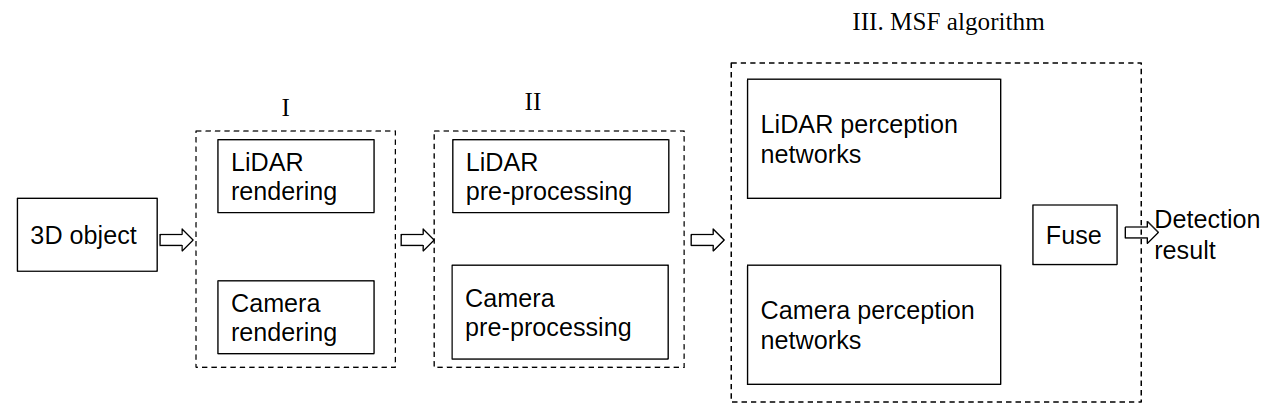
\includegraphics[width=0.8\linewidth]{figure/structure.png}
%	\caption{Perception module in AV systems}
%	\label{fig:module}
%\end{figure}
%
%\begin{figure}
%	\centering
%	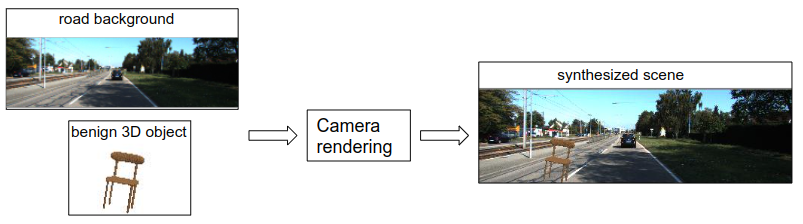
\includegraphics[width=0.8\linewidth]{figure/synthesized.png}
%	\caption{Synthesized scene through camera rendering}
%	\label{fig:synthe}
%\end{figure}
%
%\begin{figure}
%	\centering
%	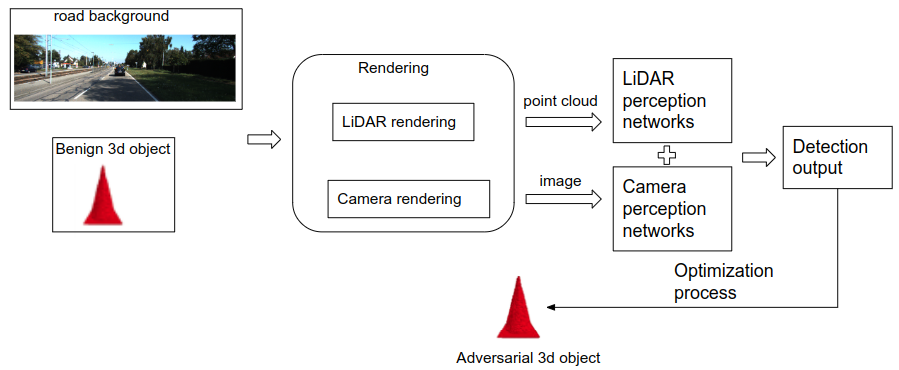
\includegraphics[width=0.8\linewidth]{figure/attack-pipeline.png}
%	\caption{Pipeline for generating adversarial 3D object attacks for both Lidar and Camera}
%	\label{fig:attack-pipe}
%\end{figure}
%------------------------


\section{Attack Model and Design Challenges}
\subsection{Attack Goal and Threat Model}
\textbf{Attack goal: Fail both LiDAR and camera perception neural networks in AV system.}
In this project, we target at evaluating the effectiveness of MSF-ADV\cite{msf-adv} attack on the synthesized scene.
The attack goal is straight-forward for affecting the safety of autonomous driving: 
fail the AV perception with LiDAR and camera sensors in the target AV, so that it can't detect the obstacle in front of it and collide with it.
This attack also assumes the AV system has the fail-safe mechanism for emergency brake. 
Even though the system is equipped with Automatic Emergency Brake(AEB), 
prior works still show that the victim vehicle can be hit by the cars behind if they fail to brake in time.
Therefore, MSF-ADV is designed for real-world physical attack with the current industry-level AD systems.

AV systems which use more than 2 perception sensors will usually be equipped with MSF algorithm,
which is to fuse the information from all of the sensors and then make decisions.
MSF still has chance to correct the wrong sensor perception as long as there is at least one clean sensor source, which is unattacked.
Since this attack aims at defeating the MSF-based AD perception, it must fail all the sensor perceptions for high attack effectiveness.
Thus MSF needs to attack all visual sensors (i.e., camera and LiDAR) at the same time.

\textbf{Threat Model.} 
MSF-ADV\cite{msf-adv} is designed in a white-box setting. 
It assumes that the attacker knows the MSF algorithm and the corresponding neural network model for each sensor perception in the target AV system.
Many prior works who study physical adversarial attacks towards sensor perception in AV systems also have similar assumptions\cite{adv1, adv2}. 
This assumption is valid as the attacker can reverse engineer the purchased or rent AV perception module to get the algorithm details.
What's more, lots of open-source industry-level AV algorithm can also be the victim, e.g., Baidu Apollo\cite{apollo}, Autoware.AI\cite{autoware}.

Since this attack is closely related to the road condition and background, 
the attacker is also assumed to take camera images and LiDAR data about the target road background to generate the adversarial objects using MSF-ADV.
After getting the adversarial object in the target background, the attacker can 3D print the object and place it at the calculated place.
To make the attack more powerful, the attacker can even fill it with high-density material like granite to make it heavier.
As a result, when the car fails to detect this object and collide with it, the damage might be more severe.
Fig. \ref{fig:noisy} shows the benign object, i.e., a chair and the malicious chair generated by MSF-ADV\cite{msf-adv}. We can notice that the surface of the malicious chair is more glitchy and it's easy for the vehicle ignore the overall shape and crash into it.

\subsection{Design Challenges}
In the state-of-art work in generating adversarial physical 3D objects,
they all use rendering functions to simulate the sensor outputs and integrate the rendering output with the road background to get the attack-influenced scenarios.
Although many works provide rendering pipelines, we find that simply feeding them with different objects and backgrounds won't meet our requirements due to 4 unique challenges:

\textbf{C1. Need to identify factors in the synthesized scene which might influence the detection accuracy of the neural network.}
To evaluate the authenticity of the synthesized scene, we need to find the factors that might make this scene more realistic or in the opposite.
However, these factors are not fully explored in prior work.
When an adversarial object is generated in previous study, they only consider certain conditions, e.g., specific background, fixed relative position.
For example, for 3d physical attacks, previous work predominantly consider the relative position between the obstacle and the target vehicle\cite{25}, 
the condition of target road background\cite{msf-adv, lidar1}. 
Although there are many other factors such as the aspect ratio of the background and light condition, 
they aren't taken into consideration in previous works when synthesizing the scene.
One possible solution is to pick different obstacles and road backgrounds as many as possible.
However, this not only adds up the testing overhead and thus decreases the testing efficiency, 
but also results in redundancy in testing cases, which might influence the trust in final results.
Thus, it is highly desired to identify some factors that can represent the difference between various synthesized scene.

\textbf{C2. Physical consistency between the obstacle and the driving background should be maximum guaranteed.} 
To ensure the synthesized scene is generated realistically in the first place, 
prior works are trying to select physically realizable object such as the drones holding cardboard with reflective surface\cite{25} and printable traffic cone\cite{msf-adv}.
Since these adversarial objects usually need a lot of optimization iterations to be generated, 
it's impractical to drive the vehicle and put the obstacle in real-life to get real-time adversarial outputs.
Therefore, most prior work will synthesize the impacts of adversarial obstacles from the physical sensor to both image and point cloud outputs, as well as integrating them into the road background.
Despite the consideration of physical realizability of the object, we also need to model the physical consistency when integrating the object and the background.
For example, no matter where we put the obstacle, it should stand on the road instead of floating in the air or even hitting the ground. 
This means we can't put the obstacle in the background with random position, instead, the physical model between the obstacle size and relative position should be established.
It should also follow the shadow caused by sunlight. 
For example, the road background is taken when there is light from the east, thus the original object in the background has the shadow facing west.
When the obstacle is put in the road, it's also supposed to have the shadow with the same direction.
Or the neural network may fail to recognize it because of the physical inconsistency.

\textbf{C3. Domain-specific metrics for quantifying the authenticity of the synthesized scene. }
In previous works designing adversarial obstacles, they adopt the optimization-based method,
an optimization loss function is designed to measure the effectiveness of the adversarial object, as well as the stealthiness of the malicious obstacle.
These loss functions are designed based on the confidence value of the object detection neural network, which reflects the probability that the region contains an object\cite{msf-adv}. 
Also they use metrics to measure the smoothness of the surface of the object.
However, these metrics are designed in a way to make the optimization process more convenient, and faster.
Our preliminary experiments show that even after the optimization, it's still possible for the neural network to detect the obstacle.
Therefore, we have to come up with new metrics to measure the performance of the object detection neural network and the adversarial attacks.
Meanwhile, previous works use different metrics to measure whether their adversarial obstacle achieves the goal and lack unified standard, 
which makes it difficult to provide fair and reasonable metrics. 

\textbf{C4. Develop an automated pipeline for generating different synthesized scenes. }
After obtaining the factors that influence the authenticity of the synthesized scenes, corresponding value ranges should be determined.
Usually the prior works only consider limited factors with certain value ranges, 
the rendering pipeline they're using may not be suitable for comprehensive testing.
It's also unrealistic to manually choose the combinations among factors as this takes a lot of effort.
Automated pipelines generating different testing scenarios should be developed.
Meanwhile, since different synthesized scenes are generated to measure its authenticity through evaluating the neural network's performance in benign and malicious cases,
this pipeline should also be equipped with neural network model inference and automatically computing the evaluation metrics along the way.
Having this automated pipeline can help us to do a large scale analysis on how realistic these synthesized scenes are.


% -----------
%\begin{figure}
%	\centering
%	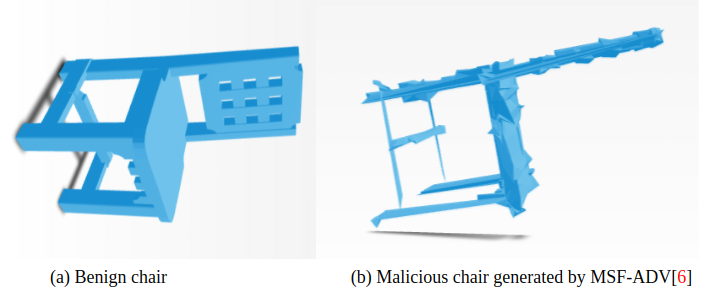
\includegraphics[width=1\linewidth]{figure/benign&ma.png}
%	\caption{Benign chair and the malicious version}
%	\label{fig:noisy}
%\end{figure}
% -----------------


\section{Approach}
In this project, we address the 4 aforementioned challenges by designing an automatic and comprehensive test suite for synthesized scenes,
which provides ways for evaluating the authenticity of the rendering methods used in MSF-ADV\cite{msf-adv}.

\subsection{Overview}

To address the challenges in Section 5.2, our test suite has the following designs;

\textbf{Different driving backgrounds, 3D obstacle properties, and their interaction}. 
To address \textbf{C1}, through our preliminary experiments, we choose driving backgrounds with different degrees of crowdedness, 
The 3D obstacle with various colors, shapes, and textures, and the relative position between the background and the obstacle.
Fig. \ref{fig:test-pipe} is the overview of the automated test suite pipeline for the synthesized scenes.

For road backgrounds, 5 different driving scenarios are chosen according to the number of cars, the light condition, the shape of the road, and the emptiness of the road.
As we can notice, some background has more than 13 cars while for others there are only 2~5 cars.
The number of cars will influence the performance of the object detection neural network as it's easier to have occlusion between the obstacle with the cars in the background when there are more cars.
The result of the neural network will be quite sensitive to the position of the obstacle when the road is more crowded.
These 5 backgrounds are with different light conditions also. 
For some backgrounds, the shadow of the trees takes up half part of the road while in other backgrounds there is less shadow on the road and even now shadows.
The shadow area will affect the object detection accuracy in a way that obstacles put in the shadow are harder to be detected, 
especially when the color of the obstacle is quite dark.

For 3D obstacle properties, we first choose different shapes of objects of the same type.
Considering that the chair is quite common and easy to obtain in real life, 
we choose the chair as our target benign obstacle and also use 3 different shapes of the chair for generality.
We also change the color and the facing angle of the chair.
The original color is wood brown, however, this is easy not to be detected when it's under shadow or close to the soil.
Therefore we also choose bright colors, i.e., blue and pink for the chair.
Also, we rotate the chair for random angles as the angles in which the chair is put will also affect the detection performance.
A chair with a full view will be detected easily while a chair with only a side view is harder to be detected and recognized as the chair.

For the interaction between the obstacle and the background, we adjust the position of the chair on both the x-axis and y-axis.
For a chair that is close to the camera, it's easier to be detected while for a chair that is far from the camera, it's the opposite case.
We implement the distance between the chair and the camera by adjusting its position on the x-axis.
The position of the chair will affect the occlusion. 
For example, if the chair is on the left side of the road and there happens to be a car here. 
The chair may block the car and prevent it to be detected.
However, if the chair is on the right side, there won't be occlusion then.

The attacker can easily simulate this by choosing an object with different shapes and colors and putting it on the road.

\textbf{Adjust the size of the object along with its position.}
To address \textbf{C2}, we adopt camera imaging theory to adjust the height of the object so that it's standing on the road.
For example, if the obstacle is far from the camera, simply cropping the obstacle image and integrating it with a farther position on the x-axis won't help.
It's likely to hit the road as the size of the obstacle should also shrink along with the increase of the distance to the camera.
In the same way, if the obstacle is close to the camera, simply moving it closer on the x-axis will likely cause the object to float in the air.
The size of the object should also increase when it's closer to the camera.
We do experiments on our backgrounds and take the following equation to model the relationship between the obstacle size and the distance between it and the camera.
\begin{equation}
	z = -1.73 + r/2
\end{equation}
Here \(z\) represents the distance between the obstacle and the camera in the unit of meters. \(r\) represents the scaling factor of the size of the obstacle.
Moving the obstacle away or closer to the camera with the corresponding scaling factor in the equation ensures 
that the obstacle is standing on the ground without floating or hitting the ground.

On the other hand, we also consider the light condition to comply with the driving background.
When there is a shadow in the background which is caused by the sunlight from a certain direction, 
an obstacle putting on the road should also have a similar shadow to ensure physical consistency.
To produce a similar light condition, 
we consider the direction and intensity of the light when we're using the camera rendering function to get the 2D image.
Also, we start with normal obstacles which can be obtained from
life easily, e.g., a common chair.
This is a fair assumption as getting the original obstacle shouldn't be difficult for the attacker.

\textbf{Detection rate and Confidence rate}
To address \textbf{C3}, we parse the output of object detection neural networks, i.e., detected bounding box, object label, and confidence scores.
Then we introduce two metrics, i.e., detection rate and confidence rate to measure the performance of the neural networks.
Specifically, Fig. \ref{fig:algo} shows the overview of the algorithm to get the total confidence scores and the correctly detected objects.
Here we choose YOLOv3 as our target neural network as it's used in Autoware.AI\cite{autoware} for object detection. 
The output of YOLOv3 includes the bounding box, label, and confidence score.
The bounding box is used to describe the position of the detected object. 
The most important part of object detection is detecting the obstacle in the right place.
Here we use the Intersection over Union(IoU) to describe the extent of overlap of two objects.
Fig. \ref{fig:iou} shows the equation to calculate IoU.
We divide the area of overlap of two objects, i.e., the ground truth bounding box and the detected bounding box, with the area of the union of two objects.
If the calculated IoU is close to 1, it means the detected bounding box almost overlaps with the ground truth and the detection position for the obstacle is correct.
We set a threshold $\alpha$ to compare with the calculated IoU to decide if the detection position is correct.

Then the label of the obstacle is chosen and compared with the ground truth label.
If they match, it means that the detected obstacle is correctly classified.
And we think this obstacle is detected correctly. 
Therefore we record the confidence score of this detection result and count this as a correctly detected object.

In the end, we use the equation in Fig. \ref{fig:detection} and Fig. \ref{fig:conf} to calculate the detection rate and confidence rate.
The detection rate is used to measure the percentage of correctly detected objects 
and the confidence rate is used to measure the average confidence scores per object.
By comparing these two metrics in synthesized scenes with different settings, 
we can evaluate the performance of the neural network and therefore the authenticity of these scenes.

\textbf{Automated pipeline for test suites} 
To address \textbf{C4}, we need to design automated pipelines for the whole testing process to improve efficiency.
In Fig. \ref{fig:test-pipe}, we first randomly choose one kind of chair as our target obstacle.
Then we randomly choose the color between wood brown, blue and pink.
The colored chair will be rotated at a random angle in [0\textdegree, 180\textdegree].
Meanwhile, a road background will be picked randomly to serve as the driving scenario.
We also shift the position of the chair on both the x-axis and the y-axis.
The shifting range in the x-axis is set to be in [4m, 8.5m] and the shifting range in the y-axis is set to be in [-8m, 8m].
While we're shifting the obstacle, we also scale the size of the object according to the camera imaging equation to ensure physical consistency.
Then we render this obstacle with a certain background to get the 2D images.
This camera image is sent to the object detection neural network to get the detection rate and confidence rate of the final outputs.
These are used to measure the authenticity of the benign synthesized image.

In Fig. \ref{fig:test-att}, we generate the adversarial obstacle using MSF-ADV\cite{msf-adv}.
Then we render the adversarial object with the camera rendering function and integrate it with the background. 
The generated 2D image is fed into the camera object detection neural network to get the detection rate and confidence rate of the adversarial synthesized scene.
This is to measure the effectiveness of generated adversarial obstacles in the road background.

%-----------


\begin{figure}
	\centering
	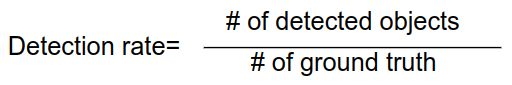
\includegraphics[width=0.7\linewidth]{figure/detection.png}
	\caption{Detection rate.}
	\label{fig:detection}
\end{figure}

\begin{figure}
	\centering
	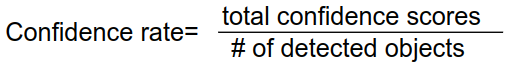
\includegraphics[width=0.7\linewidth]{figure/confidence.png}
	\caption{Confidence rate.}
	\label{fig:conf}
\end{figure}
%
\begin{figure}
	\centering
	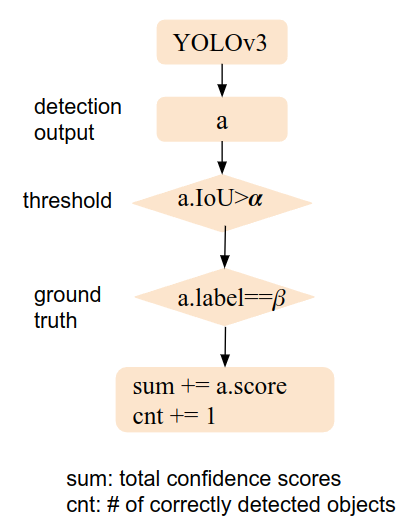
\includegraphics[width=0.5\linewidth]{figure/algorithm.png}
	\caption{Algorithm for calculating confidence scores and detected objects.}
	\label{fig:algo}
\end{figure}


\begin{figure*}
	\centering
	\begin{subfigure}{0.5\textwidth}
		\centering
		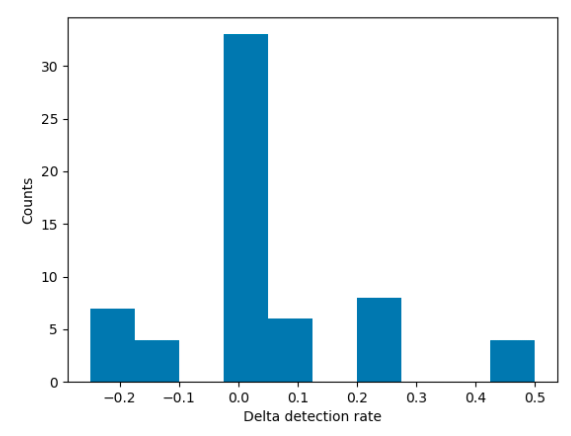
\includegraphics[width=0.7\linewidth]{figure/detection-de.png}
		\caption{Delta detection rate}
		\label{fig:det-d}
	\end{subfigure}%
	\begin{subfigure}{0.5\textwidth}
		\centering
		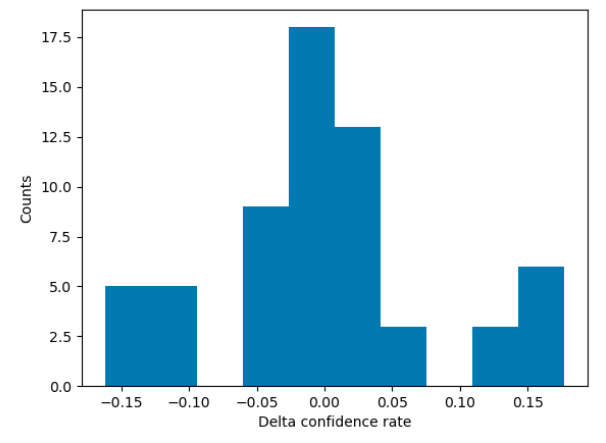
\includegraphics[width=0.7\linewidth]{figure/conf-de.png}
		\caption{Delta confidence rate}
		\label{fig:conf-d}
	\end{subfigure}
	\caption{Delta detection rate and confidence rate between benign objects and adversarial ones.}
	\label{fig:delta}
\end{figure*}

%\begin{figure*}
%	\centering
%	\begin{subfigure}{0.5\textwidth}
%		\centering
%		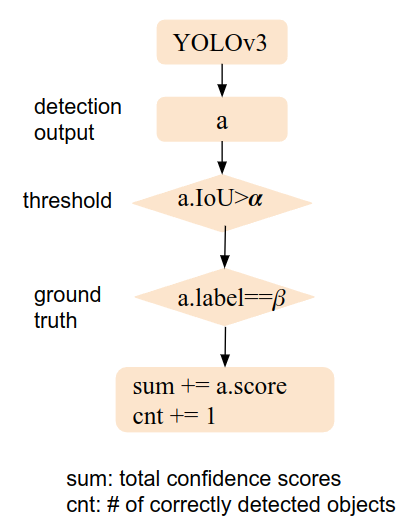
\includegraphics[width=0.7\linewidth]{figure/algorithm.png}
%		\caption{Algorithm for calculating confidence scores and detected objects.}
%		\label{fig:algo}
%	\end{subfigure}%
%	\begin{subfigure}{0.5\textwidth}
%		\centering
%		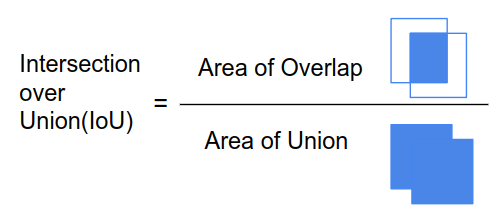
\includegraphics[width=0.7\linewidth]{figure/iou.png}
%		\caption{Intersection over Union(IoU)}
%		\label{fig:iou}
%	\end{subfigure}
%	\caption{Water treatment plant architecture and Attack Model}
%	\label{fig:swat}
%\end{figure*}

%-----------

%Adversarial 3D objects usually have noisy surfaces to mislead the detection networks.
%Thus, surface denoising is needed in the pre-processing unit.
%Directly applying the object reconstruction network like IF-Defense\cite{if-defense} will result in high computational overhead and low performance.
%Thus, we design a lightweight segmentation algorithm to first crop the potential areas containing obstacles based on laser imaging theory,
%and then apply IF-Defense\cite{if-defense} to recover the surface of the 3D object. 
%
%\subsection{Characteristics of adversarial 3D objects}
%
%Adversarial 3D objects are generated by adding, removing, and modifying the 3D points.
%These perturbations, however, will always lead to a rough object surface, violating the geometrical features in Figure~\ref{fig:noisy}(b).
%When the distance between the vehicle and the adversarial obstacle is larger than the brake distance,
%it is easy for the vehicle to mistake this glitchy surface as noise and ignore the overall shape of the obstacle.
%In this case, it fails to detect the obstacle and crashes into it.
%Therefore, it's important to smooth the noise on the surface and let the out-of-bound points lie on the surface.
%
%\subsection{Recovering methods}
%
%For 3D point clouds, there are broadly two types of methods to recover the distorted surface of 3D adversarial objects.
%One is traditional filtering based methods such as VG\cite{VG}, L0\cite{L0}, MLS\cite{mls}. They perform well in removing overall noise in the 3D perception but fail to recover the broken surfaces.
%The other is deep neural network based object reconstruction methods such as DUP-Net\cite{dupnet} and IF-Defense\cite{if-defense}.
%They aim to recover the broken surface and local part removal attack.
%
%However, they are only evaluated on a single 3D object instead of the outdoor scene perceived by autonomous cars.
%It is difficult to apply them directly in AV perception because 1) it will induce large unnecessary computation overhead as the whole road condition is fed as the input, 
%and 2) the object reconstruction methods are mostly trained on single object datasets instead of real AV outdoor datasets.
%
%Therefore, in this defense, we first design our own lightweight segmentation algorithm in real AV perception, 
%and then apply the latest object reconstruction method - IF-Defense\cite{if-defense}, to remove the noise on the surface.
%
%In the following parts, we first introduce our lightweight segmentation algorithm and then introduce the segmentation-based IF-Defense\cite{if-defense}.
%
%% For 2D images, smoothing can be done with varies filtering methods such as mean filtering\cite{mean-filter} and median filtering\cite{median-filter} 
%% and they work quite well.
%
%%% ADD figure 
%
%%\begin{figure}
%%	\centering
%%	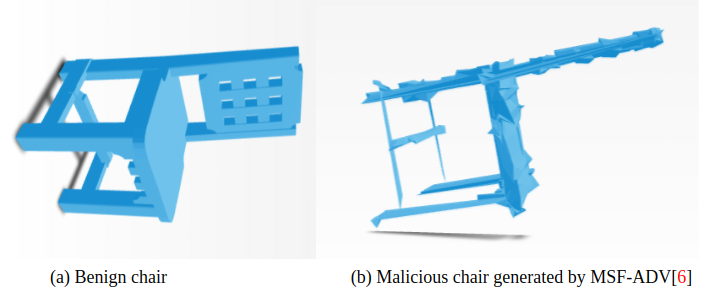
\includegraphics[width=1\linewidth]{figure/benign&ma.png}
%%	\caption{Benign chair and the malicious version}
%%	\label{fig:noisy}
%%\end{figure}
%
%% \begin{figure*}
%% 	\centering
%% 	\begin{subfigure}{0.5\textwidth}
%% 		\centering
%% 		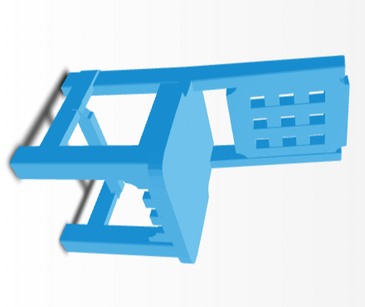
\includegraphics[width=0.6\linewidth]{figure/benign.png}
%% 		\caption{Benign chair}
%% 		\label{fig:benign}
%% 	\end{subfigure}%
%% 	\begin{subfigure}{0.5\textwidth}
%% 		\centering
%% 		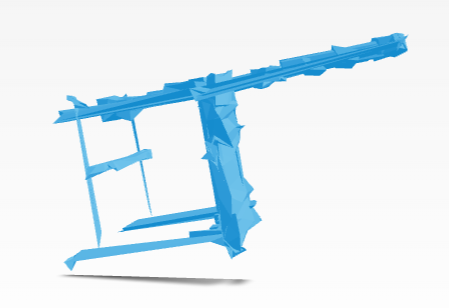
\includegraphics[width=0.7\linewidth]{figure/malicious.png}
%% 		\caption{Malicious chair generated by MSF-ADV\cite{msf-adv}}
%% 		\label{fig:noisy}
%% 	\end{subfigure}
%% 	\caption{Water treatment plant architecture and Attack Model}
%% 	\label{fig:benign&noisy}
%% \end{figure*}
%
%\subsection{Lightweight segmentation algorithm}
%
%Figure~\ref{fig:lidar} is an example of projected LiDAR perception of a traffic cone in the middle of the road. 
%These wave-like curves are the result of laser scanning in an open area.
%An obstacle will prevent the laser from scanning the area behind it and thus a blank area is formed behind the obstacle.
%We can therefore use these white areas to segment the potential areas containing the obstacle.
%After that, applying IF-Defense\cite{if-defense} only in these segmented areas will reduce the computation workload.
%
%To segment these areas, we first project the 3D object point cloud with a front view like Figure~\ref{fig:lidar} to get the image of 2D points.
%Then we divide the 2D projection into multiple cells illustrated in Figure~\ref{fig:seg}(a).
%% How to decide a?
%The cell is a square with the edge length \emph{a} to help us calculate the points' distribution. % Add figure
%We then calculate the total amount of points in the cell and store it, like in Figure~\ref{fig:seg}(b).
%Algorithm~\ref{alg:segment} shows how we get the potential segmentation areas.
%
%% We slide the cell with step \emph{d} horizontallly and vertically from one vertex to another until it walks through every 3D points.
%
%From the observation in Figure~\ref{fig:lidar}, obstacles usually have higher point density followed by a blank shadow-like area. 
%Therefore, our goal is to find dense cells which are also accompanied by a series of sparse cells.
%First, in Line 7, we sort the array of the number of points in each cell, choose the top \emph{c}\% dense cell numbers as our obstacle set \emph{A} in Line 8, and choose the least \emph{d}\% dense cell as our blank area set \emph{B} in Line 9.
%In Line 10, we select one cell \emph{i} from \emph{A}, calculate the Manhattan distance between the \emph{i} and each cell in set \emph{B} according to Eq.~\ref{eq:Manhattan}.
%
%In Eq.~\ref{eq:Manhattan}, $A(i)_x$ represents the $x$ coordinate of $i_{th}$ cell in $A$, i.e., the obstacle set.
% $A(i)_y$ represents the $y$ coordinate of $i_{th}$ cell in $A$.
% $B(i)_x$ represents the $x$ coordinate of $i_{th}$ cell in $B$, i.e., the blank area set.
% $B(i)_y$ represents the $y$ coordinate of $i_{th}$ cell in $B$.
% And the Manhattan distance $d_{ij}$ is the sum of the absolute differences of the coordinates of two points.
%We choose this metric because it's fast to calculate and also represents how far two points are from each other. 
%
%Then in Line 15, we sort the array of Manhattan distance $D$ in ascending order.
%We further calculate the Manhattan distance among the top \emph{k}\% cells in $D$ in Line 18, to measure the distances among blank area cells. 
%In Line 19, we add all the Manhattan distances in $D$ and compare it with a threshold.
%If the sum is lower than a threshold \emph{h}, we think these cells are close to each other and might be shadows of the obstacle.
%Then we choose the highest and lowest \emph{x} and \emph{y} coordinates of the points and serve this as the segmentation boundary.
%Algorithm~\ref{alg:segment} ends when all the obstacles in set A are iterated.
%We note that parameters in the algorithm like $c$, $d$, $k$, and $threshold$ have to be decided by experiment and profiling.
%
%\begin{equation}
%    \label{eq:Manhattan}
%    d_{ij} = |A(i)_x - B(j)_x| + |A(i)_y - B(j)_y|
%\end{equation}
%
%\begin{algorithm}[h]
%    \caption{Object segmentation algorithm}\label{alg:segment}
%    \begin{algorithmic}[1]
%    \State $num\_Array$: array of the number of points in each cell
%    \State $A$: obstacle sets
%    \State $B$: blank area sets
%    \State $D$: Manhattan distance array
%    \State $sum\_Dis$: Sum of difference in Manhattan distance
%    \State $bound\_Dict$: Boundaries of each segmentation
%    \State Sort $num_Array$ in descending order
%    \State $A$ $\gets$ Top c\% elements in $num_Array$
%    \State $B$ $\gets$ Least d\% elements in $num_Array$
%    % \State $p\_Array$: final pattern array
%    % \State $p\_Dict$: dictionary of detected pattern
%    % \State $idx$: the number of elements to match
%    % \State $idx \gets 2$ 
%    % \State $p \gets arrayofPac[0:1]$
%    \While{$A$ is not fully checked}
%        \While{$B$ is not fully checked}
%            \State $d_{ij}$ = |$A(i)_x$ - $B(j)_x$| + |$A(i)_y$ - $B(j)_y$|
%            \State add $d_{ij}$ into $D$
%        \EndWhile
%        \State Sort $D$ in ascending order
%        \State $D$ $\gets$ Top $k$\% $D$
%
%        \While{$D$ is not fully checked}
%            \State $diff$ = |$D(i)_x$ - $D(i+1)_x$| + |$D(i)_y$ - $D(i+1)_y$| 
%            \State $sum\_Dis$ += $diff$
%        \EndWhile
%        \If{$sum\_Dis$ < $threshold$}
%            \State $bound\_Dict[i]$ $\gets$ smallest $x$ coordinate in $D$
%            \State $bound\_Dict[i]$ $\gets$ largest $x$ coordinate in $D$
%            \State $bound\_Dict[i]$ $\gets$ smallest $y$ coordinate in $D$
%            \State $bound\_Dict[i]$ $\gets$ largest $y$ coordinate in $D$
%        \EndIf
%    \EndWhile
%    \State return $bound\_Dict$
%    \end{algorithmic}
%    \end{algorithm}
%
%\begin{figure}
%	\centering
%	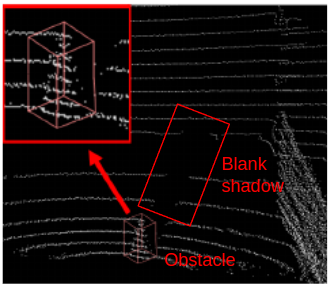
\includegraphics[width=0.5\linewidth]{figure/lidar.png}
%	\caption{LiDAR perception. Modified from Figure 10 in \cite{msf-adv}}
%	\label{fig:lidar}
%\end{figure}
%
%\begin{figure*}
%	\centering
%	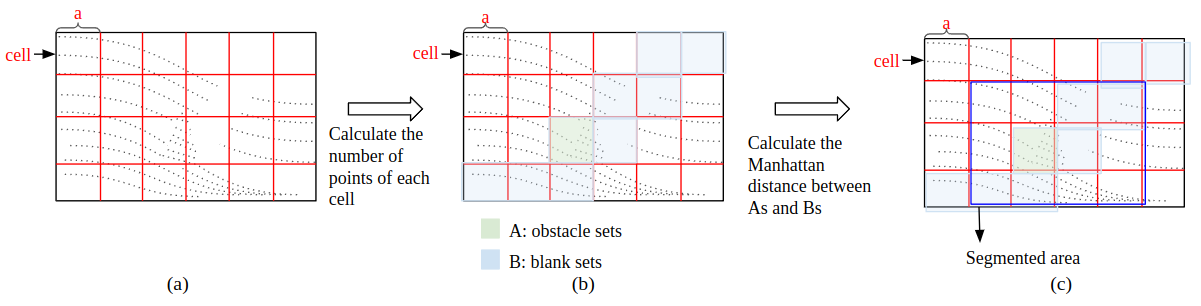
\includegraphics[width=1\linewidth]{figure/segmentation.png}
%	\caption{Segmentation algorithm}
%	\label{fig:seg}
%\end{figure*}
%
%
%
%\subsection{Segmentation-based IF-defense} 
%IF-defense\cite{if-defense} is a framework to recover the corrupted surface of the point cloud based on the implicit function\cite{implicit}.
%It aims to optimize the shape of 3D objects to follow the geometry property and realize the uniform distribution of 3D points.
%It uses geometry-aware and distribution-aware loss functions to encourage the optimized points to lie on the surface as well as distribute more evenly.
%IF-defense\cite{if-defense} is implemented with ONet\cite{ONet} and ConvONet\cite{ConvONet} network.
%However, the dataset that IF-defense\cite{if-defense} uses is ShapeNet\cite{shapenet}, which is a set of single clean 3D objects.
%It hasn't been tested on AV scenarios such as the KITTI\cite{kitti} dataset. 
%
%One big challenge of applying it on point clouds in AV outdoor perception is that there are multiple objects existing in the scene, like roads, buildings, vehicles, and pedestrians.
%Since we aim at removing the obstacle noises fed into the object detection network, recovering the whole point cloud including the road is a waste of resources.
%Also, it may not perform well in AV outdoor perception due to the different training dataset.
%
%Thus, we plan to first use the lightweight segmentation algorithm to get the potential recovery areas.
%Then we apply the IF-defense\cite{if-defense} to recover the selected areas.
%At last, we replace the originally selected point clouds with the recovered point clouds and feed the combined output into the pre-processing unit in the AV perception module. 
%In this way, we hope to recover the LiDAR detection output before sending it to the sensor fusion part.


\section{Experiments}
\subsection{Experiment setup}

For this project, we’ll use Baidu Apollo\cite{apollo} open-source AD
system. It’s a widely-used industry-grade system equipped
with the typical MSF algorithm. We’ll also use LGSVL simulator\cite{lgsvl}, an
open-source simulator providing a virtual environment to test
AV systems. To reproduce the attacks on camera and LiDAR,
we use the Github repository\cite{msf-adv} provided by Cao \emph{et al.}. After
generating adversarial objects with the tool mentioned, we’ll
test our AV-based IF-defense\cite{if-defense} by processing the rendered 3D point cloud before feeding it into the pre-processing part in Figure

As for the evaluation metric, we will measure 1) the detection accuracy of the adversarial obstacles
, 2) the detection accuracy and false-positive of the overall obstacles, including the benign ones and adversarial ones.



% \section{Discussions}
% % 1 page

\subsection{Limitations of our Experiments}
 
\subsection{Future work}

\subsection{Challenges}

\section{Related Work}
\textbf{Adversarial camera and LiDAR-based attacks AVs}
Attacks in perception sensors can be divided into two categories, camera-based attack, and object-based attack. The
camera-based attack methods\cite{7, 9, 23} propose to hide the
objects to be detected by adding adversarial patches. The attacker
can apply different interference methods to enhance the
robustness so that the objects won’t be detected from varying
observation angles and distances. This camera-based attack
aims to change the texture of the object\cite{msf-adv}. The Lidar-based
attack methods\cite{4, 6, 19, 25} propose to spoof the LiDAR with
injecting laser\cite{6}, finding vulnerable LiDAR detection locations\cite{25} or changing the shape of the 3D objects\cite{4}. This
kind of attack can fool the LiDAR object detection mechanism,
but it’s hard to spoof cameras as it aims to change the shapes
instead of the texture of the object\cite{msf-adv}. 
In these works, to mislead the neural network, some outstanding patterns are generated
to cause the model to have a tendency towards specific outputs.

\textbf{Defense towards the adversarial camera and LiDAR-based
attacks in AVs}
Defenses against these adversarial perception attacks also
fall into two types. One kind of defense\cite{if-defense, 22, 24} aims to
detect and recover the corrupted objects before they’re sent
to the detection algorithm. The authors reconstruct the objects
with implicit functions\cite{if-defense} or denoising and upsampling\cite{24}.
Although these methods can achieve a good recovering rate,
they focus on either camera-based attacks or object-based
attack. The other kind of defense aims to fuse multiple sensors\cite{10, 15, 16, 21} to avoid the spoofed sensor guiding the
detection output. These Multiple Sensor Fusion (MSF) algorithms integrate the image and LiDAR feature map 
strategically to rely on the unattacked sensors.




\bibliographystyle{plain}
\bibliography{refences}

%%%%%%%%%%%%%%%%%%%%%%%%%%%%%%%%%%%%%%%%%%%%%%%%%%%%%%%%%%%%%%%%%%%%%%%%%%%%%%%%
\end{document}
%%%%%%%%%%%%%%%%%%%%%%%%%%%%%%%%%%%%%%%%%%%%%%%%%%%%%%%%%%%%%%%%%%%%%%%%%%%%%%%%

%%  LocalWords:  endnotes includegraphics fread ptr nobj noindent
%%  LocalWords:  pdflatex acks